\section{Overview}

\begin{figure}[ht]
    \centering
    \captionsetup{justification=centering}
    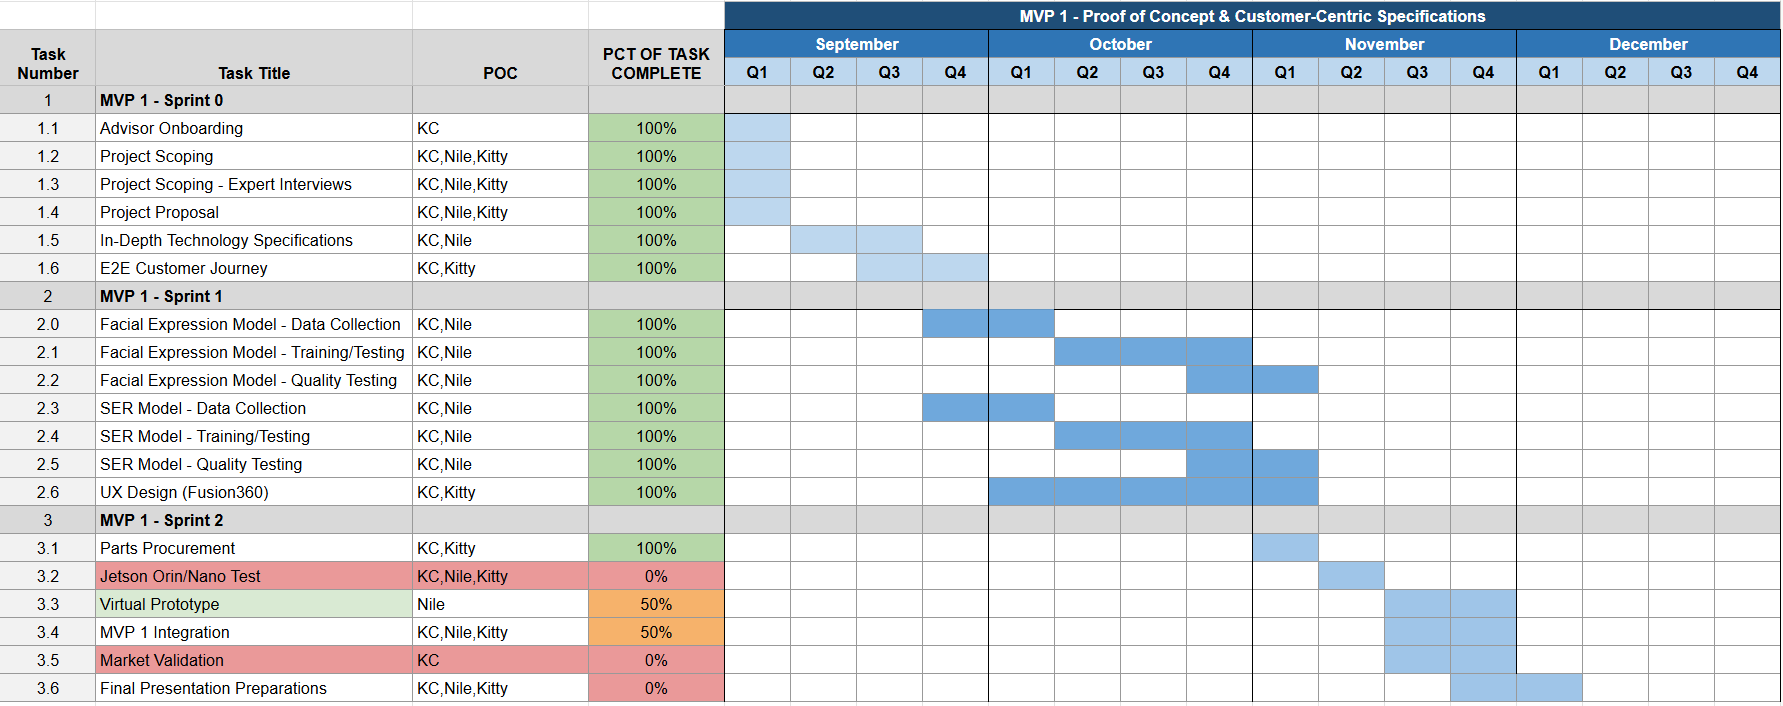
\includegraphics[width=\textwidth]{gantt.png}
    \caption{Project GANTT Chart}
    \label{fig:gantt}
\end{figure}
Overall, the project progress has taken the correct trajectory ever since the project proposal was submitted. According to the project GANTT Chart shown in Figure 1, key objectives of Q3 and Q4 (17th September to 27th September, respectively) include in-depth technology specifications and an end-to-end customer journey. In-depth technology specifications refers to the specific software approach, particularly related to machine learning, that will yield the most effective yet feasible results. On the other hand, the end-to-end customer journey refers to a flow chart for each specific interaction between human and robot, specifying the trigger points and response for the robot in order to successfully capture the objective of the project: to build a robot that can understand human emotions on a basic level, and provide positive reinforcement to alleviate signs of stress and anxiety. 